\documentclass[11pt,titlepage,twoside]{article}
\usepackage{geometry}                % See geometry.pdf to learn the layout options. There are lots.
\geometry{letterpaper}                   % ... or a4paper or a5paper or ... 
%\geometry{landscape}                % Activate for for rotated page geometry
%\usepackage[parfill]{parskip}    % Activate to begin paragraphs with an empty line rather than an indent
\usepackage{graphicx}
\usepackage{amssymb}
\usepackage{epstopdf}
\usepackage{url}
\usepackage{hyperref}
\usepackage{fancyhdr}
\DeclareGraphicsRule{.tif}{png}{.png}{`convert #1 `dirname #1`/`basename #1 .tif`.png}

\title{Microscope Simulator 2.0.0 User's Guide}
\author{Cory Quammen}
%\date{}                                           % Activate to display a given date or no date

\usepackage{fancyhdr}
\setlength{\headheight}{15pt}
 
\pagestyle{fancy}
 
\fancyhf{}
\fancyhead[LE,RO]{\thepage}
\fancyhead[RE]{\textit{Microscope Simulator 2.0.0 User Guide}}
\fancyhead[LO]{\textit{\nouppercase{\leftmark}}}
 
\fancypagestyle{plain}{ %
\fancyhf{} % remove everything
\renewcommand{\headrulewidth}{0pt} % remove lines as well
\renewcommand{\footrulewidth}{0pt}}

\begin{document}
\maketitle
\tableofcontents

\pagebreak

\section{Introduction}

The Microscope Simulator is a program for simulating the imaging process of various microscopes. Currently, simulation of fluorescence microscopes is supported through the FluoroSim module. This modules enables you to see what a geometric model of specimen would look like in a fluorescence microscope under different imaging conditions. Graphics acceleration hardware allows real time generation of simulated microscope images while you interact with specimen models.

The Microscope Simulator serves as a visual problem-solving environment with several applications:

\begin{itemize}

\item building intuition about artifacts in the imaging process by presenting the expected image from a given geometric model

\item evaluating whether a particular microscope can be used to distinguish among hypotheses in an experiment

\item checking the validity of a specimen model by comparing simulated images to experimental images from the lab

\item refining a sub-resolution estimates of a specimen model's shape by automated optimization routines

\end{itemize}

The Microscope Simulator has been designed in close collaboration with biologists to ensure the most useful features are implemented. If you have requests for features, please contact  \href{mailto:cquammen@cs.unc.edu}{Cory Quammen $\langle$cquammen@cs.unc.edu$\rangle$}.


\subsection{System Requirements}

The Microscope Simulator requires Windows XP, Windows 7, or Macintosh OS X 10.5 or higher running on an Intel processor. A recent graphics card is recommended. We have tested the Microscope Simulator on NVIDIA GeForce 8000 series graphics cards including the GeForce 8800 GTX and Quadro FX 580. More recent NVIDIA graphics cards should also be supported. The Microscope Simulator may work with ATI graphics cards, but we have not tested any. The Microscope Simulator will check the capabilities of your graphics card the first time it starts and will warn you if your graphics card is not compatible.

Your system should have at least 100 MB of hard drive space free to install the program. At least 512 MB of RAM is required, but 2 GB is recommended.

\subsection{Acknowledgements}

The Microscope Simulator is developed and maintained by the \href{http://www.cismm.org}{Center for Computer Integrated Systems for Microscopy and Manipulation}, a \href{http://www.nibib.nih.gov/}{National Institute of Biomedical Imaging and Bioengineering Resource}, award number P41-EB002025.

\section{Installation}

Installation of the Microscope Simulator is similar to installation of any other program.

\subsection{Getting the software}

To obtain the latest installer for the Microscope Simulator, visit \url{http://www.cismm.org/downloads}. Source code for the simulator is also available there.

\subsection{Windows installation}

Double-click the setup program named \textbf{MicroscopeSimulator-2.0.0-win32.exe}. On the first screen, click \emph{Next}. Please read the program license. If you agree to the terms of the license, click \emph{I Agree}. On the next screen, choose where you want to install the program. The default directory is the most-used option. Click \emph{Next}. You may optionally choose a different location in the Start Menu. By default, it will be placed in the CISMM folder. Click \emph{Install}.

\subsection{Mac installation}

Double-click the Macintosh disk image named \textbf{MicroscopeSimulator-2.0.0-darwin.dmg}. An installer program will launch and ask you to agree to the terms of the license. If you agree, a disk image named \textbf{MicroscopeSimulator-2.0.0-Darwin} will appear on your desktop and a new Finder window will open.

To install the program in your Applications directory on your computer's hard drive, drag the Microscope Simulator 2.0.0 application to either the Applications alias in the Finder window that just appeared or drag it directly to your Applications directory.

\subsection{Running the program}

\subsubsection{Windows}

You can launch the Microscope Simulator program from the Start menu. If you chose the default installation location and menu folder, select \emph{Start} $\rightarrow$ \emph{All Programs} $\rightarrow$ \emph{Microscope Simulator 2.0.0} $\rightarrow$ \emph{Microscope Simulator 2.0.0}.

\subsubsection{Macintosh}

If you installed the application in the Applications directory on your hard drive, double-click the program \emph{Microscope Simulator 2.0.0}.

\subsubsection{Running the program for the first time}

When you run the Microscope Simulator for the first time, it will run some tests to determine the capabilities of your graphics card. These tests may take a few minutes. Some graphics cards capabilities are required for the program to run while others are optional and enable certain simulation enhancements. If the optional capabilities are not present, then those simulation features will not be enabled. Currently, the only optional graphics card feature enables the generation and addition of pseudo-random Gaussian noise to simulated fluorescence images. If that feature is not available on your graphics card, the control panel section for noise will be disabled.

After the graphics card tests run, the Microscope Simulator will ask for you to choose a data directory where it can store data files. This version of the program stores one small file called \emph{PSFList.xml} which contains the list of point-spread functions defined within the program.

\section{Getting to know the Microscope Simulator}

This section gives you a tour of the many features in the Microscope Simulator.

\subsection{Program Window}

The program window, shown in Figure \ref{fig:ProgramWindow}, consists of several panels. A standard menu bar appears at the top of the window (Windows) or in the system menu bar. Below the menu bar is the \emph{Simulator Control Panel} where settings for the microscopes can be edited. The large panel in the center of the window showing a blue color gradient and grid of white lines is the \emph{Model Display Panel} where specimen models are displayed. Rotating, translating, and scaling models interactively with the mouse also takes place in this window. A row of icons above the \emph{Model Display Panel} controls how specimen models appear and whether simulation results are superimposed with the models. The \emph{Model Settings Control Panel} on the right consists of two parts; the \emph{Model Object List} at the top displays a list of models in the simulation, and the \emph{Model Object Properties Panel} at the bottom displays a list of model properties that can typically be edited. Each of these panels is described in more detail below.

\begin{figure}[htbp] %  figure placement: here, top, bottom, or page
   \centering
   \includegraphics[width=1\linewidth]{images/ProgramWindow-small} 
   \caption{The program window after startup.}
   \label{fig:ProgramWindow}
\end{figure}

\subsection{Menu Bar}

The menu bar in the Microscope Simulator contains five menus that provide commands useful to creating new simulations, adding specimen models to a simulation, saving simulations, and loading saved simulations, among other actions. Each menu is described in more detail below.

\subsubsection{File Menu}

The \emph{File Menu} features typical options for creating and saving simulations:

\begin{description}
  \item[New Simulation] \hfill \\
  Creates a new simulation with default settings.

  \item[Open Simulation...] \hfill \\
  Opens a saved simulation file.

  \item[Save Simulation] \hfill \\
   Saves a simulation's settings to a file. This includes the settings of each microscope simulator, the objects in the scene and their settings, and everything else required to recreate the simulation. If the simulation has not been saved previously, you will be asked to provide a name and location for the file.
   
  \item[Save Simulation As...] \hfill \\
  Does the same thing as the \emph{Save Simulation} menu item, but allows you to save the simulation to another file name.
  
  \item[Exit] \hfill \\
  Exits the program. \textbf{Macintosh users:} The \emph{Quit} menu item appears under the \emph{MicroscopeSimulator} menu instead of the \emph{File} menu.

\end{description}

\subsubsection{Edit Menu}

The \emph{Edit Menu} contains functions common to many programs.

\begin{description}

  \item[Cut] \hfill \\
  \emph{Currently not implemented}
  
  \item[Copy] \hfill \\
  \emph{Currently not implemented}
  
  \item[Paste] \hfill \\
  \emph{Currently not implemented}

\end{description}

\subsubsection{Model Menu}
\label{sec:ModelMenu}

The \emph{Model Menu} has options for adding and removing geometric models to the simulation. Every model in this menu has parameters that controls its shape. Models are placed at the center of the simulation domain.

\begin{description}

  \item[Add Cylinder] \hfill \\
  Adds a model of a cylinder to the simulation. The ends of the model are capped with flat ends. The length and radius of the tube can be changed.
  
  \item[Add Hollow Cylinder] \hfill \\
  Adds a model of a cylinder with a hollow center to the simulation. Like the cylinder model, the length and outer radius of the tube can be changed. A separate parameter controls the thickness of the tube walls where thickness is defined as the difference between the diameter of the outer and inner cylinder walls.

  \item[Add Disk] \hfill \\
  Adds a model of a planar disk to the simulation. The disk is defined by its center and a radius.

  \item[Add Flexible Tube] \hfill \\
  Adds a model of tube to the simulation. The tube is defined by several control points and a radius. The number of control points can be changed, and each control point can be specified independently.
  
  \item[Add Plane] \hfill \\
  Adds a simple bounded planar model to the simulation. The plane is defined by its width and height.
  
  \item[Add Point Ring] \hfill \\
  Adds a set of an arbitrary number of points to the simulation. The points are restricted to lie in a circle of a given radius. These positions are treated as mathematical points in the simulator, so they are suitable for simulating very small objects such as nanometer-sized particles. No geometry is involved, but the points are represented by small spheres in the \emph{Model Object Window} so that they can be seen easily.
  
  \item[Add Point Set] \hfill \\
  Adds a set of an arbitrary number of points to the simulation. This model is the same as the point ring, but the points are not restricted to lie in a circle. The location of each point can be set independently.
  
  \item[Add Sphere] \hfill \\
  Adds a sphere model to the simulation. The radius of the sphere can be changed.

  \item[Add Torus] \hfill \\
  Adds a torus to the simulation. The radius of the torus and the radius of the cross-section can be adjusted independently.

\end{description}

\subsubsection{Import Menu}

\begin{description}

  \item[Import Image Data...] \hfill \\
  Imports an image file. Single TIFF (2D and 3D) and LSM (Zeiss) files can be imported. You will typically use this when importing an image file to which models should be fit using FluoroSim.
  
  \item[Import Geometry File...] \hfill \\
  Imports geometry from a file. Supported files include:
  
  \begin{itemize}
  \item VTK Files (*.vtk)
  \item VTK Poly Data XML Files (*.vtp)
  \item OBJ Files (*.obj)
  \item PLY Files (*.ply)
  \end{itemize}

\end{description}

\subsubsection{Window Menu}

\begin{description}

  \item[About] \hfill \\
  Shows a window with information about the Microscope Simulator program. \textbf{Macintosh users:} The \emph{About Microscope Simulator} menu item appears under the \emph{Microscope Simulator} menu instead of the \emph{Window} menu. 

  \item[Show Simulator Control Panel] \hfill \\
  Shows/hides the \emph{Simulator Control Panel}. If you close the \emph{Simulator Control Panel}, you can show it again with this menu item.
  
  \item[Show Model Settings Control Panel] \hfill \\
    Shows/hides the \emph{Model Settings Control Panel}. If you close the \emph{Model Settings Control Panel}, you can show it again with this menu item.
  
  \item[Show Fluorescence Window] \hfill \\
  Shows/hides a separate panel that displays the fluorescence images simulated by FluoroSim.
  
  \item[Show Errors] \hfill \\
  Displays a window listing any errors in the program.
  
  \item[Preferences] \hfill \\
  Displays the \emph{Preferences Window} (see Section \ref{sec:PreferencesWindow}).

\end{description}

\begin{figure}[htbp] %  figure placement: here, top, bottom, or page
   \centering
   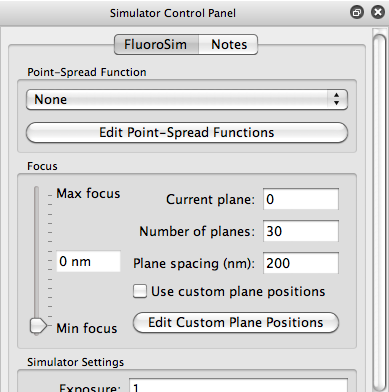
\includegraphics[width=3in]{images/SimulatorControlPanel} 
   \caption{The \emph{Simulator Control Panel} with the \emph{FluoroSim Tab} selected.}
   \label{fig:SimulatorControlPanel}
\end{figure}

\subsection{Simulator Control Panel}

This control panel has two tabs. The \emph{FluoroSim Tab} contains controls for fluorescence simulation. More details on these controls are available in the FluoroSim section of this manual (Section \ref{sec:FluoroSim}). The \emph{Notes Tab} contains a text editor where notes about the current simulation may be written. These notes will be saved in the simulation file and will be loaded when the simulation file is loaded.

\subsection{Model Display Panel}

The \emph{Model Display Panel} is where the 3D specimen models in the simulation are displayed. Output from the Microscope Simulator modules can also be displayed in this window. Such output include fluorophores generated by FluoroSim and fluorescence images superimposed in among the specimen models.

\subsection{Visualization Buttons}

\begin{figure}[htbp] %  figure placement: here, top, bottom, or page
   \centering
   
\includegraphics[width=4in]{images/VisualizationIcons} 
   \caption{Cisualization controls. Starting from the left: \emph{Save Model Object Image}, \emph{Reset Camera}, \emph{View Model Objects Only}, \emph{View Fluorophore Sampling}, \emph{References Axes Button}, \emph{Move Camera}, and \emph{Move Objects}.}
   \label{fig:VisualizationControls}
\end{figure}

A row of visualization icons provide various controls related to what is shown in the \emph{Model Display Panel} (see Figure \ref{fig:VisualizationControls}). The functions represented by the icons are described from left to right below:

\subsubsection{Utility Buttons}

\begin{description}

  \item[Save Model Object Image] \hfill \\
  Save the image currently displayed in the \emph{Model Object Panel}.
  
  \item[Reset Camera] \hfill \\
  Reset the scene to the default view.
  
\end{description}

\subsubsection{Visualization Buttons}

Just one of the following visualization modes can be enabled at a time:

\begin{description}

  \item[View Model Objects Only] \hfill \\
  Displays specimen models only.

  \item[View Model Objects and Fluorophore Sampling] \hfill \\
  Displays fluorophores from models in the scene as small spheres.

%  \item[View Models with AFM Scan] \hfill \\
%  Displays both the specimen models and the simulated AFM surface scan.

  %\item[View AFM Scan Only] \hfill \\
  %Displays the simulated AFM surface scan only.
  
  %\item[View Models with Fluorescence Comparison] \hfill \\
  %Displays comparison of experimental and simulated fluorescence image stacks with the models visible. See the section on processing simulated stacks for more details on the comparison visualization.
  
  %\item[View Fluorescence Comparison Only] \hfill \\
  %Display comparison of experimental and simulated fluorescence image stacks without the models visible. See the section on processing simulated stacks for more details on the comparison visualization.
  
\end{description}
  
\subsubsection{References Axes Button}

Enables/disables display of coordinate axes in the \emph{Model View Panel}. The location of the coordinate axes can be moved to an arbitrary location in the \emph{Model View Panel} display by clicking on the axes and dragging them.
  
\subsubsection{Interaction Modes Button}
\label{sec:InteractionModesButton}
  
One of the following interaction modes can be enabled at a time.

\begin{description}

  \item[Move Camera] \hfill \\
  Enables manipulation of the camera in the Model View Panel via mouse manipulation. You can change the view of the specimen models by rotating, translating, and zooming in on the scene. Clicking and dragging while holding different mouse buttons causes different camera motions:

\begin{itemize}
\item \textbf{Left mouse button} - rotates the scene
\item \textbf{Middle mouse button} - translates the scene
\item \textbf{Right mouse button} - zooms in on the scene
\end{itemize}

  \item[Move Objects] \hfill \\
  Enables manipulation of individual specimen model objects via mouse manipulation. Clicking on the desired model object and dragging while holding one of the mouse buttons produces the following transformations:
  
\begin{itemize}
\item \textbf{Left mouse button} - rotates the selected model object
\item \textbf{Middle mouse button} - translates the selected model object
\item \textbf{Right mouse button} - in most cases, scales the size of the model object
\end{itemize}

\end{description}

\subsection{Model Object List}

The model object list appears in the upper right of the program window. All model objects in the simulation are listed here. When you click on a model object in the list, properties for that model object appear in the Model Object Properties Panel. Right-clicking on a model object brings up a context menu that provides several options:

\begin{description}

  \item[Focus on Object] \hfill \\
  Changes the camera view to center on this model object and zoom in on it so that it nearly fills the Model Object View Panel.
  
  \item[Export Geometry] \hfill \\
  Exports the model object geometry as a VTK Legacy file (*.vtk), VTK Poly Data XML file (*.vtp), PLY file (*.ply), or BYU file (*.byu).
  
  \item[Delete Model Object] \hfill \\
  Deletes this model object.

\end{description}

\begin{figure}[htbp] %  figure placement: here, top, bottom, or page
   \centering
   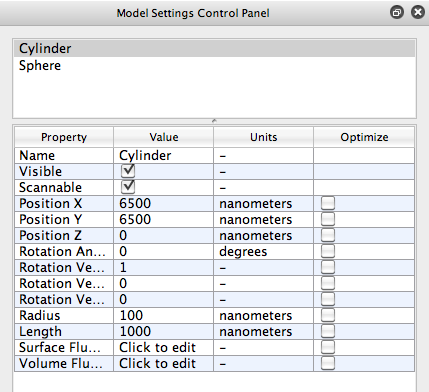
\includegraphics[width=3in]{images/ModelObjectProperties} 
   \caption{The \emph{Model Settings Control Panel}. The \emph{Model Object List} (top section) shows all the specimen models in the simulation. The \emph{Model Object Properties List} (bottom section) contains an editable list of the selected model object's properties.}
   \label{fig:example}
\end{figure}

\subsection{Model Object Properties Panel}

\subsubsection{The Properties Table}

The \emph{Model Object Properties Panel} has four columns showing the properties of the model object selected in the \emph{Model Object List}. Each property is displayed as a row in the table. Most model object properties can be changed in this panel, but some are there to display information about the model object (the size in voxels of an \emph{Image Model Object}, for example).

The \emph{Property} column lists the name of the property. Property names cannot be edited. The \emph{Value} column lists the value of the property. To change the value, click on the table cell. Clicking on a property with a checkbox will toggle the checkbox. Clicking once on a property with a numerical value will select the cell while clicking it twice will highlight the value; in either case, typing a numerical value and pressing the return key will change the property value. The \emph{Units} column shows the units of the parameter and cannot be edited. Unitless properties are denoted with a dash (``-''). The \emph{Optimize} column contains checkboxes to designate which property should be optimized using FluoroSim's model fitting routines (see Section \ref{sec:ModelFittingToFluorescenceImages}).

\subsubsection{Common Model Object Properties}

A few properties common to almost all model objects are listed here:

\begin{description}

  \item[Name] \hfill \\
  A name for the model object.
  
  \item[Visible] \hfill \\
  Controls whether the model object is visible in the scene or not.

  \item[Scannable] \hfill \\
  Controls whether the model object is included when calculating a simulated AFM scan. \emph{Not yet implemented.}

  \item[Position X] \hfill \\
   X-component of the model object position.

  \item[Position Y] \hfill \\
  Y-component of the model object position.

  \item[Position Z] \hfill \\
  Z-component of the model object position.
  
  \item[Rotation Angle] \hfill \\
  Angle of rotation in rotation about the vector defined by the next three parameters.
  
  \item[Rotation Vector X] \hfill \\
  X-component of the vector about which the model is rotated.
  
  \item[Rotation Vector Y] \hfill \\
  Y-component of the vector about which the model is rotated.
  
  \item[Rotation Vector Z] \hfill \\
  Z-component of the vector about which the model is rotated.
  
  \item[Surface Fluorophore Model] \hfill \\
  A fluorophore model that samples the surface of the specimen model geometry (see Section \ref{sec:FluorophoreModels}).
  
  \item[Volume Fluorophore Model] \hfill \\
  A fluorophore model that samples the volume defined by boundaries of the specimen model geometry (see Section \ref{sec:FluorophoreModels}).

\end{description}

\subsection{Preferences Window}
\label{sec:PreferencesWindow}

\begin{figure}[htbp] %  figure placement: here, top, bottom, or page
   \centering
   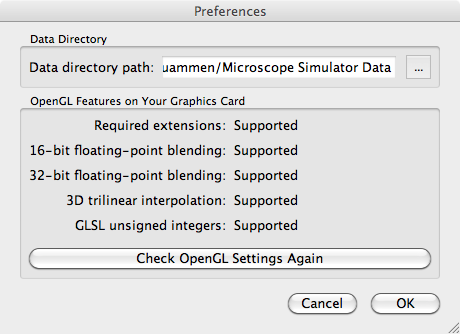
\includegraphics[width=4in]{images/PreferencesWindow} 
   \caption{The Preferences window.}
   \label{fig:PreferencesWindow}
\end{figure}

The \emph{Preferences Window} (Figure \ref{fig:PreferencesWindow}) lets you specify a directory where the Microscope Simulator can store data files. This directory was set the first time the program ran, but it can be changed by clicking on the button to the right of the directory.

The required and optional graphics card capabilities are also listed in the \emph{Preferences Window}. If you install the Microscope Simulator and later upgrade your graphics card, you can check the capabilities of the new card by clicking the \emph{Check OpenGL Settings Again} button. This will also enable the advanced capabilities of the Microscope Simulatorthe when you restart the program.

\section{FluoroSim}
\label{sec:FluoroSim}

FluoroSim is a Microscope Simulator module for fluorescence microscope simulation. From the model objects in the scene, FluoroSim computes the image that would be expected in a fluorescence microscope. Different microscopes can by simulated by selecting different point-spread functions (PSFs), each of which characterize the optics of a microscope.

\subsection{Image Formation Model}

A fluorescence microscope can be modeled as a linear system. As such, an image $I$ is formed by the convolution of the true signal $S$ from the fluorescing molecules in the specimens with the point-spread function (PSF) $H$ that characterizes the optics of the microscope. Mathematically, image formation is modeled by the equation:

\begin{equation}
I = S \otimes H
\end{equation}
where $\otimes$ denotes the convolution operator. In FluoroSim, $S$ is a set of mathematical points in 3D Cartesian space that is automatically generated by a particular type of model object property called a fluorophore model (see Section \ref{sec:FluorophoreModels}). FluoroSim currently simulates image formation in incoherent systems only. 

\subsection{Noise Model}

FluoroSim can also simulate additive noise in fluorescence images. Noise in comes from several sources in the microscope. Shot noise arises from fluctuations in the number of photons emitted from the fluorophores in the specimen and detected by the CCD elements in the camera, background noise comes from stray photons in the system, and read-out noise comes from the CCD electronics.

The various noise sources follow different probability distributions. Taken together, their effects can be often be approximated by a Gaussian distribution. The fluorescence microscope simulator models noise according to a Gaussian distribution, adding the noise to the result of the convolution of the fluorophores with the PSF. The final image formation model, then, is:

\begin{equation}
I = S \otimes H + N
\end{equation}
where $N$ is the modeled noise. 

\subsection{Point-Spread Function Controls}

\begin{figure}[htbp] %  figure placement: here, top, bottom, or page
   \centering
   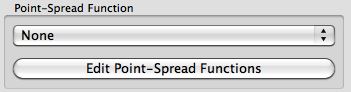
\includegraphics[width=4in]{images/FluoroSim/PointSpreadFunctionControls} 
   \caption{Point-Spread Function controls.}
   \label{fig:PointSpreadFunctionControls}
\end{figure}

A critical component of generating realistic simulated fluorescence images is the PSF of the microscope. FluoroSim lets you create a list of PSFs characterizing the different microscopes you use. PSFs you have defined appear in the pop-up menu in the \emph{Point-Spread Function} controls (see Figure \ref{fig:PointSpreadFunctionControls}). The pop-up menu let's you choose which point-spread function (PSF) to use. The \emph{Edit Point-Spread Functions} let's you edit PSF properties.

\subsection{The Point-Spread Function Editor}

\begin{figure}[htbp] %  figure placement: here, top, bottom, or page
   \centering
   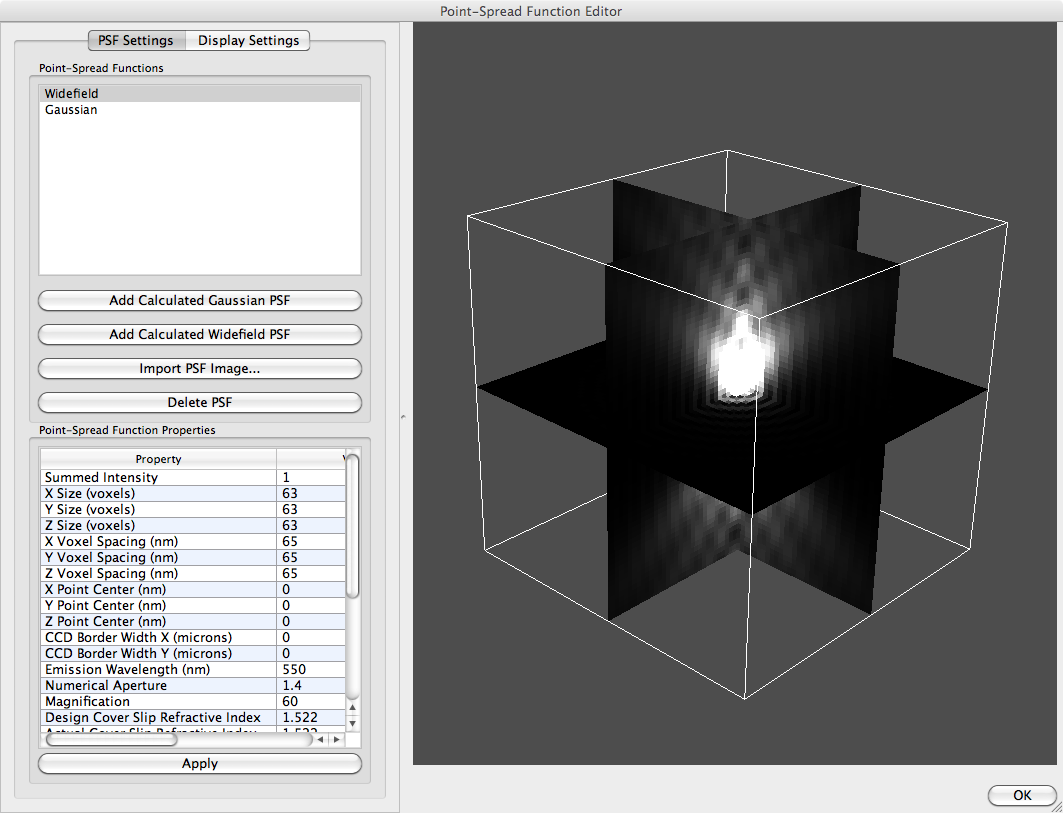
\includegraphics[width=4.5in]{images/FluoroSim/PSFEditor} 
   \caption{The PSF Editor window.}
   \label{fig:PSFEditor}
\end{figure}

When you click on the \emph{Edit Point-Spread Functions} button, a new window called the \emph{Point-Spread Function Editor} appears as shown in Figure (\ref{fig:PSFEditor}). This window has a control panel on the left side and a visualization panel for displaying PSFs on the right side.

The top half of the control panel lists the available PSFs. To select a PSF to visualize and edit, click on the name of the PSF in the PSF list. To rename a PSF, double-click on its entry in the PSF list, type the new name, and press the return key.

\subsubsection{Adding and Deleting PSFs}
\label{sec:AddingAndDeletingPSFs}

Four buttons below the PSF list enable adding and deleting PSFs:

\begin{description}

\item[Add Calculated Gaussian PSF] \hfill \\
A 3D Gaussian is often used to model the PSF of a confocal microscope. The parameters of this model include the standard deviation of the Gaussian in each of the three spatial dimensions.

\item[Add Calculated Widefield PSF] \hfill \\
Gibson and Lanni\footnote{Gibson, S. F. and Lanni, F. (1992 ). Experimental test of an analytical model of aberration in an oil-immersion objective lens used in 3-D microscopy. \emph{Journal of the Optical Society of America}, 9(1):154�166.} proposed a model for aberrated PSFs in widefield microscopes. This model assumes that an objective lens has been designed for specific microscope parameters. When the actual parameters of the microscope match the design parameters, an ideal PSF is formed. When the actual parameters do not match, the difference in the length of the path traveled by a ray in the design system and a ray in the actual system causes a phase shift that leads to an aberrated PSF. This model parameters include: emission wavelength, numerical aperture, magnification, design and actual cover slip refractive indices, design and actual cover slip thicknesses, design and actual immersion oil refractive indices, design immersion oil thickness, design and actual specimen layer refractive indices, depth in specimen layer, and the design and actual distances from the back focal plane.

\item[Import PSF Image...] \hfill \\
A PSF image generated from an external program may be imported by clicking on this button. 3D TIFF and Zeiss LSM files can be imported.

\item[Delete PSF] \hfill \\
To delete a PSF, select it in the PSF list and click this button.

\end{description}

\subsubsection{Changing PSF Model Properties}
\label{sec:ChangingPSFModelProperties}

The bottom half of the control panel features a property table showing the properties of the PSF selected in the PSF list. The \emph{Property} column provides the name of the property and its unit of measurement where appropriate. The \emph{Value} column gives the property value. To edit a value, double-click its table entry, type in the new value, and press the return key. After editing property values, you must click the \emph{Apply} button to make the changes take effect. If you click on a different PSF. If you close the window before clicking the \emph{Apply} button, then re-open the window, your changes will still appear in the property table, but will not yet have been applied to the PSF model.

A column of property values may be pasted into the \emph{Value} column. To do so, copy a column of property values (single numerical entries separated by line endings) to the system clipboard, double-click the property corresponding to the first value in the column of values you copied, and type Control-V (Command-V on the Mac).

PSF property values may also be copied  from the \emph{Value} column by clicking on one property value, holding down the shift key, clicking another property value, and typing Control-C (Command-C on the Mac).

\subsubsection{Common PSF Model Properties}

Several properties are common to all PSF models:

\begin{description}

\item[Summed intensity] \hfill \\
The summed intensity is the integrated intensity value over the entire PSF.

\item[X Size (voxels)] \hfill \\
The number of voxels in the $x$-direction.

\item[Y Size (voxels)] \hfill \\
The number of voxels in the $y$-direction.

\item[Z Size (voxels)] \hfill \\
The number of voxels in the $z$-direction.

\item[X Voxel Spacing (nm)] \hfill \\
The spacing between voxels in the $x$-direction.

\item[Y Voxel Spacing (nm)] \hfill \\
The spacing between voxels in the $y$-direction.

\item[Z Voxel Spacing (nm)] \hfill \\
The spacing between voxels in the $z$-direction.

\end{description}

\subsubsection{Visualizing the PSF}

Two tabs appear at the top of the control panel in the \emph{Point-Spread Function Editor} window. The \emph{PSF Settings} tab holds the controls described in Sections \ref{sec:AddingAndDeletingPSFs}--\ref{sec:ChangingPSFModelProperties}. The \emph{Display Settings} tab provides controls for visualizing the selected PSF (see Figure \ref{fig:PSFEditorDisplaySettings}).

The \emph{Image Planes} controls affect the placement of slice planes through the PSF volume. Three such planes are provided, spanning the $x-$, $y-$, and $z-$planes. The checkbox next to each plane controls whether the plane is visible, the number of the slice plane determines which slice is displayed, and the slider bar can be used to change the position of the slice plane.

The \emph{Contrast} controls determine how the intensity values in the PSF map to the screen. Clicking on the \emph{Reset Levels} button resets the controls so that the smallest intensity maps to black and the greatest intensity maps to white. The slider bars can be used to adjust both the min and max levels.

The \emph{Camera} controls consist of six buttons that move the camera to six canonical positions. The +X button moves the camera to look down the positive $x$-axis and the -X button move the camera to look down the negative $x$-axis. The -Y, +Y, -Z, and +Z have similar functions, but operate on different coordinate axes.

The mouse may be used to interact to change the position of the camera in the the PSF display panel on the right side of the screen. The controls are identical to the controls in the \emph{Model Display Panel} (see Section \ref{sec:InteractionModesButton}).

\begin{figure}[htbp] %  figure placement: here, top, bottom, or page
   \centering
   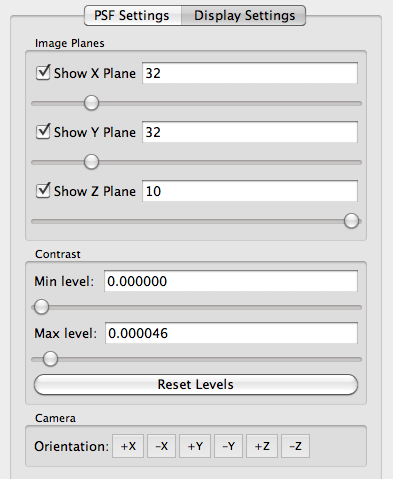
\includegraphics[width=4in]{images/FluoroSim/PSFEditorDisplaySettings} 
   \caption{Display Settings in the \emph{Point-Spread Function Editor}.}
   \label{fig:PSFEditorDisplaySettings}
\end{figure}

\subsection{Focus Controls}

FluoroSim generates fluorescence images one focal plane at a time. In some applications, a single focal plane is sufficient as it emulates the operation of a real microscope. In other applications where simulation of optical sectioning is required to produce 3D images of the specimen, a number of focal plane positions must be defined. 

Each focal plane is referenced by an index, and the \emph{Current plane} shows which plane is being used to generate the simulated image (see Figure \ref{fig:FluoroSimFocusControls}). The \emph{Number of planes} determines how many focal planes are in the 3D volume, and the \emph{Plane spacing} determines the spacing between subsequent focal planes.

The focal plane index can be set through either the slider on the left side or the \emph{Current plane} text box. Focal plane indices start at 1. The physical focal depth corresponding to a focal plane index is displayed to the right of the focus slider.

In some microscopes, the specimen stage may not travel the same distance in $z$ between every adjacent focal plane. If the stage reports the actual distance traveled between focal planes, this distance can be entered into FluoroSim by clicking on the \emph{Edit Custom Plane Positions} button. The \emph{Focal Plane Positions} window will be shown as in Figure \ref{fig:FocalPlanePositions}. The column on the left displays the focal plane index while the column on the left shows the focal plane position in nanometers. By default, all focal plane positions are at position 0 nanometers. The \emph{Reset} button below the table of focal plane positions can be used to populate the table with evenly-spaced focal plane positions that can then be modified by double-clicking the table cell, typing the new position, and pressing the return key.

\begin{figure}[htbp] %  figure placement: here, top, bottom, or page
   \centering
   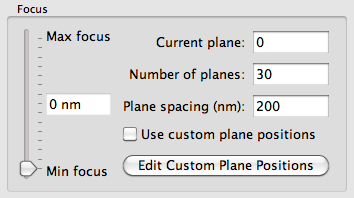
\includegraphics[width=4in]{images/FluoroSim/FocusControls} 
   \caption{Focus Controls}
   \label{fig:FluoroSimFocusControls}
\end{figure}


\begin{figure}[bp] %  figure placement: here, top, bottom, or page
   \centering
   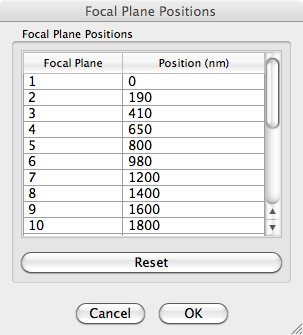
\includegraphics[width=3in]{images/FluoroSim/FocalPlanePositions} 
   \caption{Focal Plane Positions window.}
   \label{fig:FocalPlanePositions}
\end{figure}

\subsection{Simulator Settings}

test

\begin{figure}[htbp] %  figure placement: here, top, bottom, or page
   \centering
   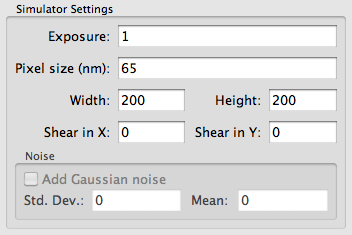
\includegraphics[width=4in]{images/FluoroSim/SimulatorSettings} 
   \caption{Simulator Settings controls.}
   \label{fig:FluoroSimSimulatorSettingsControls}
\end{figure}

\subsubsection{Image Controls}

\subsubsection{Noise} 

\subsection{Fluorescence Display}

\begin{figure}[htbp] %  figure placement: here, top, bottom, or page
   \centering
   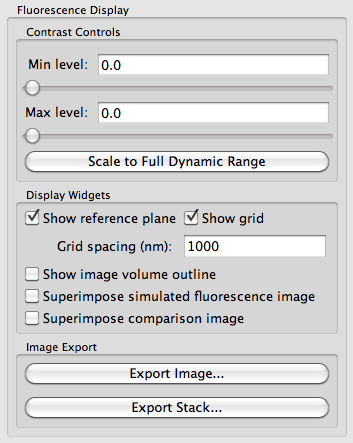
\includegraphics[width=4in]{images/FluoroSim/FluorescenceDisplay} 
   \caption{Fluorescence Display controls}
   \label{fig:FluoroSimFluorescenceDisplayControls}
\end{figure}

\subsubsection{Contrast Controls}

\subsubsection{Display Widgets}

\subsubsection{Image Export}

\subsection{Model Fitting}

\begin{figure}[htbp] %  figure placement: here, top, bottom, or page
   \centering
   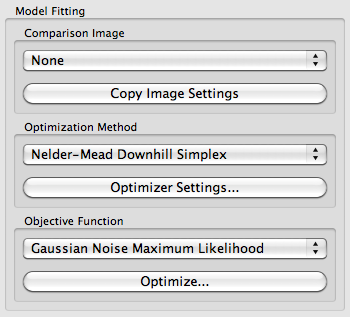
\includegraphics[width=4in]{images/FluoroSim/ModelFitting} 
   \caption{Model Fitting controls.}
   \label{fig:FluoroSimModelFittingControls}
\end{figure}

\subsubsection{Comparison Image}

\subsubsection{Optimization Method}

\subsubsection{Objective Function}


\subsection{Fluorophore Models}
\label{sec:FluorophoreModels}

A \emph{fluorophore model} provides a way to model fluorescent labeling as it occurs at the molecular level. Most model objects have one or more fluorophore models that control aspects of the fluorophore sampling process. There are two primary kinds of fluorophore models, surface models and volume models. In surface models, point samples are taken from the surface of the model object geometry. Volume models sample the volume defined within an enclosing geometry. Volume sampling requires the surface geometry of a model object to form an enclosed volume; objects that do not have this property cannot be sampled with a volume fluorophore model. \footnote{A third type of fluorophore model applies does not perform random sampling of the geometry but instead uses explicitly defined fluorophore locations specified by the model. This type of fluorophore model is used by only the \emph{Point Ring} and \emph{Point Set} model objects (see Section \ref{sec:ModelMenu} for details on these model objects).}

\begin{figure}[htbp] %  figure placement: here, top, bottom, or page
   \centering
   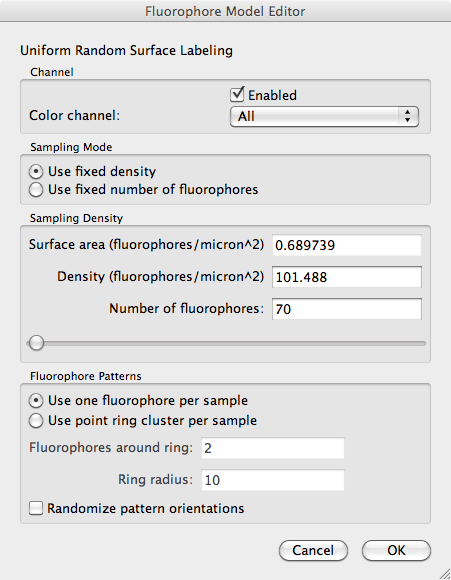
\includegraphics[width=4in]{images/FluoroSim/FluorophoreModelEditor} 
   \caption{The Fluorophore Model Editor for a surface fluorophore model.}
   \label{fig:FluorophoreModelEditor}
\end{figure}

Both kinds of models can be edited in the \emph{Fluorophore Model Editor}. Figure \ref{fig:FluorophoreModelEditor} shows the editor for a surface fluorophore model. The controls for the editor are organized into four different sections.

\subsubsection{Channel}

The \emph{Channel} controls let you choose whether the fluorophore model is enabled in the simulation and in which color channel it should appear. The control panel items to do this are:

\begin{description}

\item[Enabled] \hfill \\
When checked, this check box indicates that the fluorophores generated by this model are visible in the simulated fluorescence image.

\item[Color channel] \hfill \\
This menu lets you select the color channel(s) in which the fluorophores should appear. The color channels are red, green, blue, or all (red, green, \emph{and} blue).

\end{description}

\subsubsection{Sampling Mode}

The \emph{Sampling Mode} controls let you decide whether either the density of the sampling should be fixed or the number of samples should be fixed. 

\begin{description}

\item[Use fixed density] \hfill \\
Use a fixed spatial density of samples. When selected, the fluorophore model will preserve the approximate density of the fluorophore sampling when the total surface area (or volume) changes because of a change in a shape parameter value. The total number of fluorophore samples may increase or decrease.

\item[Use fixed number of fluorophores] \hfill \\
Use a fixed number of samples. When selected, the fluorophore model will preserve the number of fluorophores sampled from the geometry. Changes to a shape parameter will not affect the total number of fluorophore samples, but the density may increase or decrease.

\end{description}

\subsubsection{Sampling Density}

The \emph{Sampling Density} controls let you control the density of the fluorophore sampling or the absolute number of samples taken on the geometry.

\begin{description}

\item[Surface area (Volume)] \hfill \\
Specifies the surface area (or volume) of the portion of the model object on which the fluorophore model operates. Not editable.

\item[Density] \hfill \\
Specifies the density of the fluorophore sampling. The specified density does not necessarily reflect the density of samples in a local portion of the geometry because random sampling does not generally produce an even distribution of samples. Instead, this figure represents the average density over the geometry. Furthermore, because an integer number of fluorophore samples are taken, only a discrete number of densities can be accurately represented for a given surface area or volume. The actual average sampling density is effectively rounded to the nearest representable density below the desired density.

\item[Number of fluorophores] \hfill \\
Specifies the number of fluorophores sampled from the geometry. This number is linked to the density through the surface area (or volume) of the geometry.

\end{description}

\subsubsection{Fluorophore Patterns}

In certain applications, it can be useful to model fluorophores as a particular pattern at each sample location instead of a single fluorophore. These controls let you determine which pattern to use and their properties.

\begin{description}

\item[Use one fluorophore per sample] \hfill \\
When selected, places a single fluorophore at each sample.

\item[Use point ring cluster per sample] \hfill \\
When selected, places a point ring at each sample position. The number of fluorophores around the ring and the radius of the ring can be specified. Randomization of the ring orientation can also be enabled.

\end{description}

\subsubsection{Fixed Fluorophore Model}

Because the \emph{Fixed Fluorophore Model} does not sample the geometry, only the \emph{Channel} controls are available (see Figure \ref{fig:FixedFluorophoreModelEditor}). Fluorophore patterns for this model are not supported.

\begin{figure}[htbp] %  figure placement: here, top, bottom, or page
   \centering
   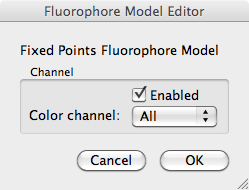
\includegraphics[width=2.5in]{images/FluoroSim/FixedFluorophoreModelEditor} 
   \caption{The Fluorophore Model Editor for a fixed fluorophore model.}
   \label{fig:FixedFluorophoreModelEditor}
\end{figure}

\subsection{Model Fitting to Fluorescence Images}
\label{sec:ModelFittingToFluorescenceImages}


%\pagebreak

\section{Version History}

\subsection{Version 2.0.0}

\noindent
Changes from previous release:
\begin{itemize}
\item Complete rewrite of the Microscope Simulator program.
\end{itemize}

\noindent
Known issues:
\begin{itemize}
\item Item
\end{itemize}

\end{document}  